Unlike in previous years, this course is intended to be a stand-alone course on general relativity, building up the mathematical formalism needed to construct the full theory and explore some examples of interesting spacetime metrics. It is linked to the Black Holes course taught in Lent term, which I will also be writing notes for.

Some recommended course materials and readings include the following:
\begin{itemize}
\item Sean Carroll, Spacetime and Geometry\footnote{I should point out that Sean Carroll's textbook is based off a set of GR notes which are available for free online. They are really excellent and pedagogically structured, and I have cross-referenced them frequently when revising these notes after lecture. Here is a link to the PDF on the arXiv: \url{https://arxiv.org/pdf/gr-qc/9712019.pdf}}
\item Misner, Thorne, and Wheeler, Gravitation
\item Wald, General Relativity
\item Zee, Einstein Gravity in a Nutshell
\item Hawking and Ellis, ``The Large Scale Structure of Spacetime''
\end{itemize}

In Minkowski\footnote{I've heard some USAmericans pronounce this ``min-cow-ski.'' In German, it is ``min-koff-ski.''} spacetime (flat space) we specify points in spacetime by spatial coordinates in $\RR^3$, i.e. the Cartesian coordinates $(x,y,z)$, plus a time coordinate $t$. The line element (spacetime separation) is given by the metric
$$ds^2=-dt^2+dx^2+dy^2+dz^2.$$
$ds$ is the proper distance between $x$ and $x+dx$, $y$ and $y+dy$, $z$ and $z+dz$, and $t$ and $t+dt$. (As is typical in relativity, we work in units where $c=1$. Note that the metric sign convention here is flipped from my QFT notes, which uses the ``mostly minus'' convention-- this is arbitrary and so long as one is consistent it makes no difference.) Using the Einstein summation convention, the metric is usually written more compactly as $$ds^2=\eta_{\alpha\beta}x^\alpha x^\beta,$$ with $\eta_{\alpha\beta}$ the Minkowski space metric.

Let's recall from special relativity that we call separations with $ds^2>0$ ``spacelike,'' with $ds^2<0$ ``timelike,'' and $ds^2=0$ null (or occasionally lightlike).
\begin{defn}
The \term{chronological future} of a point $p$ is the set of all points that can be reached from $p$ along future directed timelike lines, and we call this $I^+(p)$. It is the interior of the future-directed light cone. Conversely we have the chronological past of $p$, $I^-(p)$, which is the interior of the past-directed light cone. We also have the \term{causal future} of $p$, which is the set of all points that can be reached from $p$ along future-directed timelike \emph{or} null lines, and we call this $J^+(p)$. Similarly we have the causal past, $J^-(p)$. Thus $J$ is the closure of $I$ and is the interior \emph{plus} the light cone itself.
\end{defn}

\begin{figure}
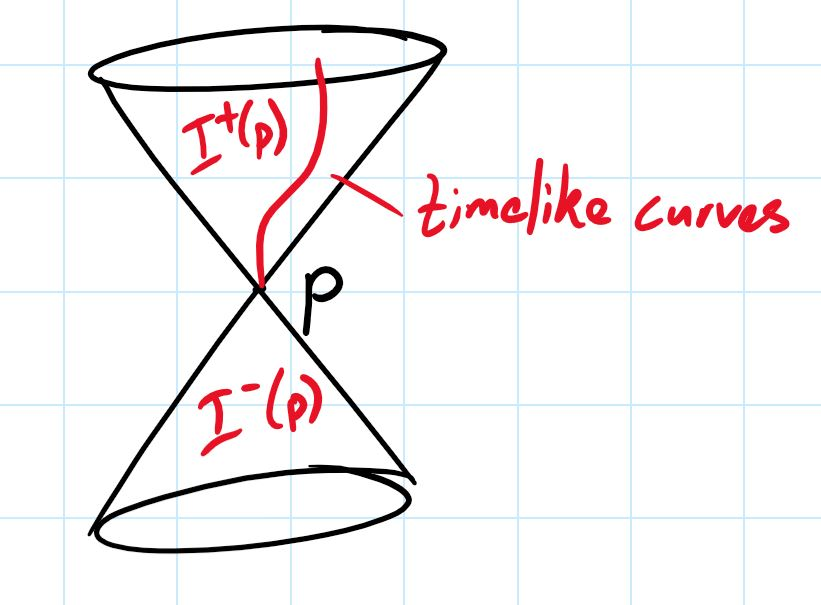
\includegraphics[width=0.5\textwidth]{2018/10/20181005_img1}
\caption{An illustration of the light cones from a point $p$, plus the chronological future $I^+$ and chronological past $I^-$. Also depicted in red is a timelike curve (e.g. a possible particle trajectory in spacetime).}
\end{figure}

Let $x^a(\tau)$ be a curve in spacetime.\footnote{Evidently we are not using the convention that Greek indices range from $0$ to $3$ and Latin indices range from $1$ to $3$. I have copied the lecturer's convention here, but may change to more traditional notation if it becomes relevant.} Then the tangent vector to the curve is $u^a=\frac{dx^a}{d\tau}$. For timelike curves, $u^a u^b \eta_{ab}=-1 \iff \tau$ is the proper time along the curve.
\footnote{The property that $U^\alpha U^\beta \eta_{\alpha\beta}=-1$ is easy to prove. See the Special Relativity catch-up sheet found \href{http://www.maths.cam.ac.uk/sites/www.maths.cam.ac.uk/files/grspecialrelativity.pdf}{here} for some nice exercises in SR: this is exercise 3. Assuming the result of exercise 2 which states that the four-velocity of a massive particle is $U^\mu=\gamma(1,v^i)$, we then have $U\cdot U =\gamma^2(-1+v^2)=\frac{v^2-1}{1-v^2}=-1$. Since this is a fully contracted expression (no indices floating around), it is true in all frames.}
We also know that $\int_p^q d\tau = \Delta \tau$, which just says that the integral of $d\tau$ along a curve from $p$ to $q$ yields the proper time interval, what a clock actually measures.

We also remark that Minkowski space has some very nice symmetries. Since $x,y,$ and $z$ do not appear explicitly in the metric, our spacetime is invariant under translations. It is also invariant under rotations in $\RR^3$. It would be nice to extend rotations to include the time coordinate $t$ as well-- this is exactly what a Lorentz transformation does.

Lorentz transformations in general involve time-- they are defined by the matrices $\Lambda$ which satisfy
$$\Lambda^T \eta \Lambda= \eta,$$
i.e. they preserve the inner product $\eta$ in Minkowski space, forming the group $O(3,1)$. Lorentz transformations consist of rotations in $\RR^3$ and boosts. This is equivalent to the defining property of rotation matrices $R$ that $R^T \delta R=\delta$, meaning that rotation matrices preserve the standard Euclidean inner product in $\RR^3$ and form the group $O(3)$.\footnote{Strictly, $O(3)$ also includes reflections-- for matrices which preserve both orientation and the inner product, we must also require that $\det R=+1$, defining the group $SO(3)$. We'll see a similar caveat with the Lorentz group in just a second.}
Written explicitly, the Lorentz boost in the $x$-direction to a frame moving with velocity $v$ is
\begin{align*}
t&\to t'=\frac{t-vx}{\sqrt{1-v^2}}\\
x&\to x'=\frac{x-vt}{\sqrt{1-v^2}}\\
y&\to y'=y\\
z&\to z'=z
\end{align*}
We may also write it in matrix notation,
$${\Lambda^a}_b =
\begin{pmatrix}
\gamma&-\gamma v &0 & 0\\
-\gamma v & \gamma & 0 & 0\\
0&0&1&0\\
0&0&0&1
\end{pmatrix}$$
where $\gamma$ is defined in the usual way by $\gamma \equiv \frac{1}{\sqrt{1-v^2}}$.

Rather than constructing the (in general complicated) Lorentz boost in an arbitrary direction, it is often more convenient to rotate one's frame of reference in $\RR^3$ so the boost is in the new $x$-direction, perform the Lorentz boost, and then transform back:
$$R^T \Lambda R= \Lambda_R,$$
where $\Lambda_R$ is a new Lorentz transformation.\footnote{It's easy to check that $\Lambda_R$ really is a Lorentz transformation-- just observe that rotations alone are a subset of Lorentz transformations, since they preserve the inner product on $\RR^3$ and do not affect the time coordinate. In the language of group theory, rotations form an $SO(3)$ subgroup of the full Lorentz group $O(3,1)$-- see Definition \ref{lorentzgroup}. Therefore any combination of rotations and Lorentz boosts will form another valid Lorentz transformation by the group closure property.}

\begin{defn}\label{lorentzgroup}
The Lorentz transformations taken together form the \term{Lorentz group}. It satisfies the group axioms of identity, unique inverses (since $\det\Lambda \neq 0$), associativity (from associativity of matrix multiplication), and closure (see footnote for proof).\footnote{More precisely, we know that the determinant is nonzero since $-1=\det{\eta}=\det(\Lambda^T\eta\Lambda)=\det(\Lambda^T)\det(\eta)\det(\Lambda)=(-1)\det(\Lambda)^2\implies \det(\Lambda)=\pm 1 \neq 0$. To prove closure, suppose $\Lambda_1,\Lambda_2$ are Lorentz transformations. The product $\Lambda_1\Lambda_2$ then satisfies $(\Lambda_1\Lambda_2)^T \eta(\Lambda_1\Lambda_2)= \Lambda_2^T \Lambda_1^T \eta\Lambda_1 \Lambda_2 = \Lambda_2^T \eta \Lambda_2 = \eta$, so $\Lambda_1\Lambda_2$ is also a Lorentz transformation.}
\end{defn}

$\Lambda$ can include reflections in time or space. To avoid such complications, we sometimes refer to the \term{proper orthochronous Lorentz group,} i.e. to exclude space and time reversals, but often we are more careless and simply call it the Lorentz group.
\begin{defn}
The \term{Poincar\'e group} is then the semidirect product of Lorentz transformations and translations. This is the group of symmetries of Minkowski space.
\end{defn}
We have translations defined as
$$x^a\to {x^a}'=x^a+\Delta x^a$$
and also Lorentz transformations, with the property
$${(\Lambda^T)_a}^c \eta_{cd} {\Lambda^d}_b=\eta_{ab}.$$


\begin{defn}
We also have \term{contravariant vectors} (indices up) written $u^a$ and their corresponding \term{covariant} vectors (indices down) $$u_a\equiv\eta_{ab}u^b,$$ where we have used the metric to lower an index. These are sometimes equivalently called simply vectors and covectors. We can also raise indices using the inverse metric $\eta^{ab}$ (defined by $\eta^{ab}\eta_{bc}=\delta^a_c$). Thus
$$u^b=\eta^{ba}u_a.$$
\end{defn}

We define the Lorentz transformation of a contravariant vector as
$u^a\to {u^a}' = {\Lambda^a}_b u^b.$  For instance, $x^a$ is an example of a contravariant vector.

\begin{defn}
A \term{scalar} is an object which is invariant under a Lorentz transformation. We saw that a covariant vector transforms with right multiplication by the Lorentz transformation, whereas a contravariant vector transforms by left multiplication. 

More generally, a \term{tensor of type $(r,s)$} transforms with $r$ copies of the Lorentz transformation on the $r$ up indices and $s$ copies of the Lorentz transformation on the $s$ down indices, 
\begin{equation}
{T^{\mu_1 \mu_2\ldots \mu_r}}_{\nu_1 \nu_2 \ldots \nu_s} \to {T^{\alpha_1 \alpha_2\ldots \alpha_r}}_{\beta_1 \beta_2 \ldots \beta_s}=\Lambda^{\alpha_1}_{\mu_1} \ldots \Lambda^{\alpha_r}_{\mu_r} {T^{\mu_1 \mu_2\ldots \mu_r}}_{\nu_1 \nu_2 \ldots \nu_s} \Lambda^{\nu_1}_{\beta_1}\ldots \Lambda^{\nu_s}_{\beta_s}
\end{equation}

By this definition, a scalar may be thought of as a type $(0,0)$ tensor, a contravariant vector a type $(1,0)$ tensor, and a covariant vector a type $(0,1)$ tensor.
\end{defn}